% ----------------------------------------------------------
\chapter{Comportamento Mecânico de Túneis}
% ----------------------------------------------------------

\section{Influência da escavação e o conceito de convergência da seção}

De uma forma geral, do ponto de vista do maciço, a escavação de um túnel nada mais é do que uma perturbação no seu estado natural de equilíbrio devido à remoção de parte do maciço. Essa perturbação induzirá o maciço a uma nova configuração de equilíbrio que mobilizará tensões tangenciais desviando, dessa forma, a direção das tensões principais no entorno da escavação. Através desse \textbf{arqueamento das tensões}, o próprio maciço participa da sustentação da cavidade. Esse arqueamento pode ser decomposto em dois arcos longitudinais (contidos nos planos horizontal e vertical) e um arco transversal (no plano perpendicular ao eixo do túnel), tal como mostrado na \autoref{arqueamento}.

\begin{figure}[H]
	\begin{center}
		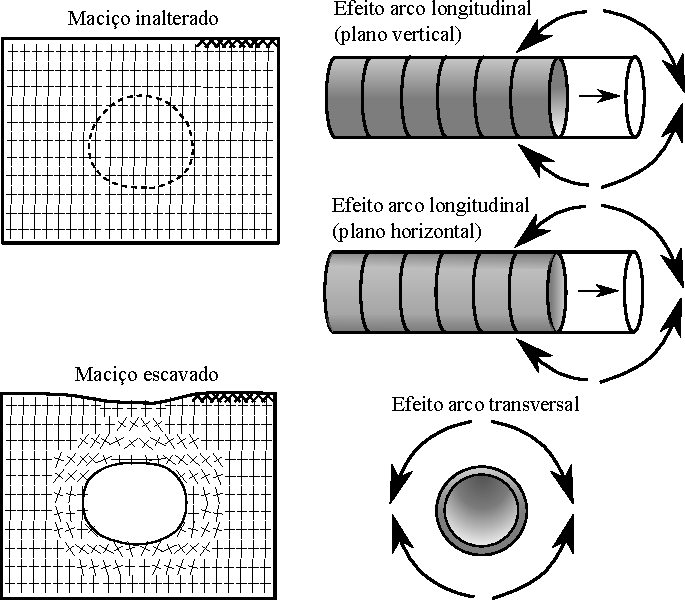
\includegraphics[scale = 1]{0401-efeito_arco.pdf}
	\end{center}
	\caption{\label{arqueamento}Ilustração do arqueamento das tensões principais (adaptado de: \citeonline[p. 10-11]{Franca2006})}
\end{figure}

A presença dos três arcos na zona que acompanha a frente de escavação faz com que essa região tenha um campo de deslocamentos tridimensional convergente em direção à face de escavação. No entanto, conforme essa frente avança e se afasta, apenas o arqueamento transversal se mantém, fazendo com que o campo de deslocamentos seja bidimensional contido no plano transversal ao eixo do túnel. Em vista disso, é conveniente caracterizar três zonas no interior do maciço: uma zona não perturbada pela escavação, uma zona de influência da frente de escavação e uma zona livre dessa influência (\autoref{campo_frente_escavacao}).

\begin{figure}[H]
	\begin{center}
		\includegraphics[scale = 1]{0402-campo vetorial de deslocamentos no maciço.pdf}
	\end{center}
	\caption{\label{campo_frente_escavacao}Campo vetorial de deslocamentos no maciço durante a escavação de um túnel (adaptado de: \citeonline[p. 12]{Franca2006})}
\end{figure}

O parâmetro geométrico mais simples e representativo do comportamento de um túnel é o fechamento de sua cavidade, também conhecido como \textbf{convergência}. Se um túnel circular estiver em um maciço homogêneo, isotrópico, submetido a um estado de tensões inicial geostático hidrostático, o campo de deslocamentos no entorno de uma seção fora da zona de influência da frente de escavação estará contido no plano transversal e será puramente radial, podendo ser expresso por uma função  $u(r)$. Nesse caso, a convergência $U$ é definida pela razão entre o deslocamento da cavidade e seu raio inicial $U=-u(r=R)/R$. A presença do sinal negativo é opcional e serve para que a convergência fique positiva se a seção diminuir, ou seja, $u(R) < 0$  (\autoref{definicao_convergencia}).

\begin{figure}[H]
	\begin{center}
		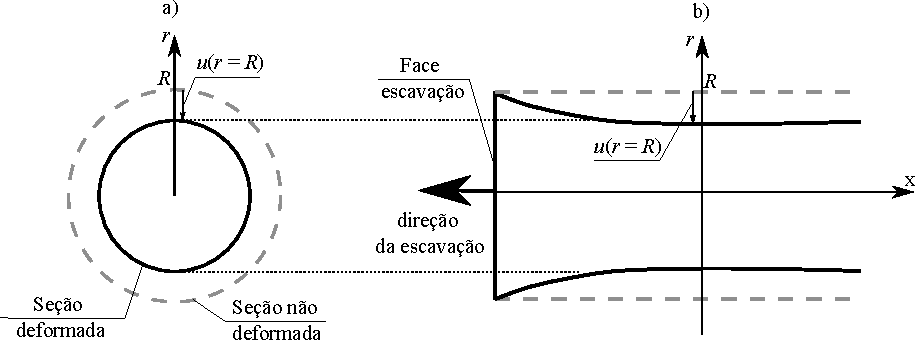
\includegraphics[scale = 1]{0403-convergencia de uma seção circular.pdf}
	\end{center}
	\caption{\label{definicao_convergencia}Ilustração das medidas geométricas que compõe a convergência de uma seção circular: a) corte transversal, b) corte longitudinal}
\end{figure}

Dependendo da anisotropia das tensões \textit{in situ} ou do formato da seção, sua deformada pode não ser radial e, na prática, podem-se usar varias medidas para compor o cálculo da convergência da seção, como exemplificado na \autoref{convergenca_secao_qualquer}.

\begin{figure}[H]
	\begin{center}
		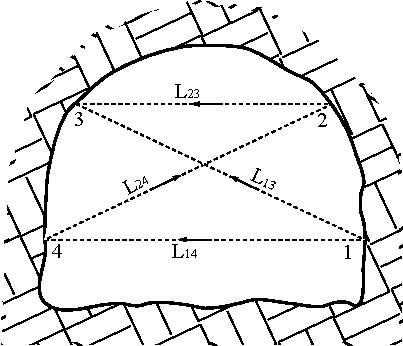
\includegraphics[scale = 1]{0404-convergencia de uma seção qualquer.pdf}
	\end{center}
	\caption{\label{convergenca_secao_qualquer}Medidas da convergência em quatro direções de uma seção não circular (adaptado de: \citeonline[p. 8]{Panet1995})}
\end{figure}

Outro aspecto importante para determinar a influência da escavação e caracterizar o comportamento global do túnel é a representação gráfica das convergências ao longo do seu eixo longitudinal, conhecida como \textbf{perfil de convergências}. Por exemplo, com o objetivo de quantificar a extensão da zona de influência da frente da escavação, Hanafy \& Emery (1980) graficaram o perfil de convergências do seu modelo de um túnel circular em um maciço homogêneo, isotrópico e elástico linear (\autoref{perfil_exemplo}).

\begin{figure}[H]
	\begin{center}
		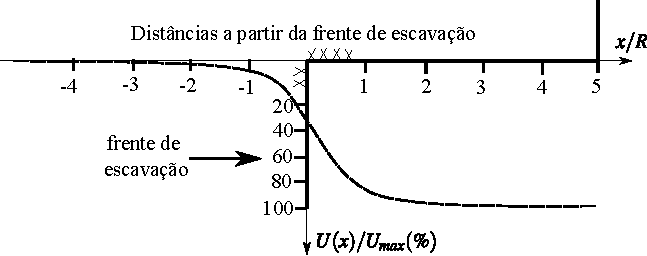
\includegraphics[scale = 1]{0405-perfil de convergencias próximo a frente de escavação.pdf}
	\end{center}
	\caption{\label{perfil_exemplo}Perfil de convergências próximo à frente de escavação (adaptado de: \citeonline{Hanafy1980} \textit{apud} \citeonline[p. 42]{Couto2011})}
\end{figure}

Como se pode ver na \autoref{perfil_exemplo}, dentro das hipóteses dos autores, a partir de cinco raios da face de escavação a convergência atinge seu valor máximo  $U_{max}$. Já na face, em $x/R=0$ , a convergência é superior à 35\% do valor máximo, sendo que a um raio de distância a convergência é de aproximadamente 80\% da total e quase 100\% se tiver ultrapassado dois raios (\citeonline{Hanafy1980} \textit{apud} \citeonline[p. 42]{Couto2011}).

\section{Mecanismos de ruptura em túneis profundos}

A execução de túneis se tornou bastante segura após os preceitos filosóficos e teóricos do método empírico NATM (\textit{New Austrian Tunneling Method}) desenvolvido por Rabcewicz (\citeyear{Rabcewicz1964a}, \citeyear{Rabcewicz1964b} e \citeyear{Rabcewicz1964c}) e \citeonline{Rabcewicz1973}. E cada vez mais os estudos numéricos vêm ajudando os projetistas na tomada de decisões seguras durante a fase de projeto e execução. Contudo, apesar dessa abordagem empírica e numérica ter diminuído significativamente o número de incidentes estes ainda existem. Compilados de acidentes podem ser encontrados em estudos da \citeonline{HealthandSafetyExecutiveHSE1996} e de pesquisadores como \citeonline{Stallmann2005}, \citeonline{Seidenfus2006} e \citeonline{Sousa2010}, tal como reunido por \citeonline{Spackova2012} na \autoref{incidentes}.

\begin{figure}[H]
	\begin{center}
		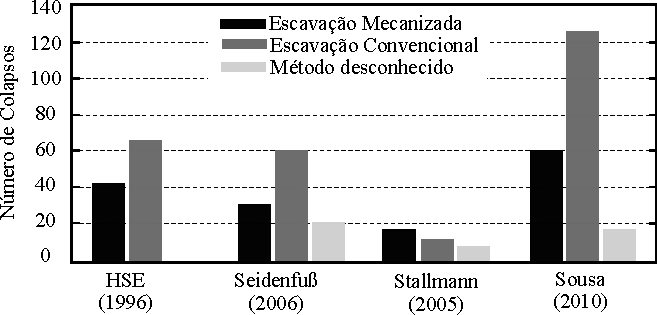
\includegraphics[scale = 1]{0406-número de incidentes em quatro banco de dados descriminado por autor e tecnologia de escavação.pdf}
	\end{center}
	\caption{\label{incidentes}Número de incidentes em quatro banco de dados descriminados por autor e método de escavação (adaptado de: \citeonline[p. 19]{Spackova2012})}
\end{figure}

\citeonline{Sousa2010}, por exemplo, agrupou os incidentes, tanto de túneis profundos como superficiais, em nove tipos, tal como apresentado na \autoref{distribuicao_incidentes}.

\begin{figure}[H]
	\begin{center}
		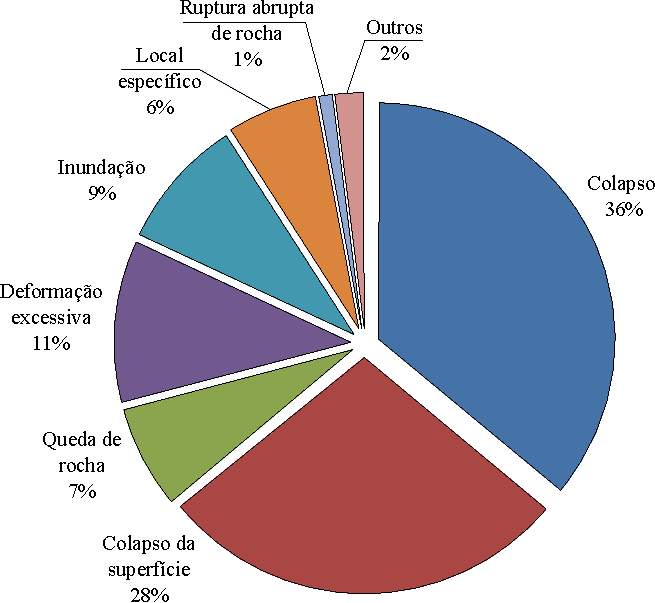
\includegraphics[scale = 1]{0407-distribuição de incidentes de acordo com nove tipologias.pdf}
	\end{center}
	\caption{\label{distribuicao_incidentes}Distribuição de incidentes de acordo com nove tipologias (adaptado de: \citeonline[p. 82]{Sousa2010})}
\end{figure}

Contudo, de forma geral, no comportamento de túneis profundos executados em maciços aparentemente contínuos, ou seja, ausência de grandes descontinuidades ou acidentes geológicos, identifica-se dois mecanismos principais de colapso (ou ruptura): \textit{Spalling} (descamação ou fragmentação) e \textit{Squeezing} (deformações excessivas diferidas no tempo).

O \textit{Spalling} é preponderante em maciço muito resistente, inicialmente pouco fraturado, no qual o nível de energia para iniciar a fissuração e consequente propagação costuma ser alto. Durante a redistribuição das tensões, causada pela escavação, as fissuras vão se desenvolvendo e destacando regiões da rocha no contorno da seção. Essas sofrem então uma descamação, ou ainda, ruptura por flambagem e tem-se, nesse último caso, uma repentina liberação de energia. Uma ruptura abrupta da rocha (\textit{rockburst}). Esse comportamento é refletido na curva tensão-deformação de uma amostra do maciço, por um significativo amolecimento após o pico de resistência, caracterizando, dessa forma, a rocha como frágil \cite[p. 83]{Kleine2007}. A \autoref{mecanismo_spalling} exemplifica esse mecanismo e a \autoref{foto_spalling} mostra a seção após tal colapso.

\begin{figure}[H]
	\begin{center}
		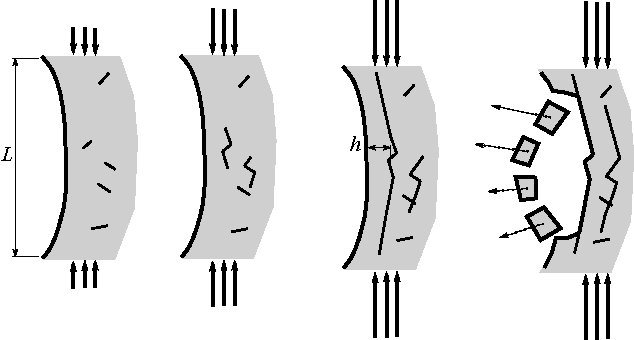
\includegraphics[scale = 1]{0408-mecanismo de ruptura do maciço próximo a seção.pdf}
	\end{center}
	\caption{\label{mecanismo_spalling}Mecanismo de ruptura por \textit{Spalling} de um comprimento $L$ junto à seção do túnel: detalhamento do crescimento das fissuras e flambagem de uma profundidade $h$ da rocha no contorno da seção (adaptado de: \citeonline[p. 267]{Germanovich2000})}
\end{figure}

\begin{figure}[H]
	\begin{center}
		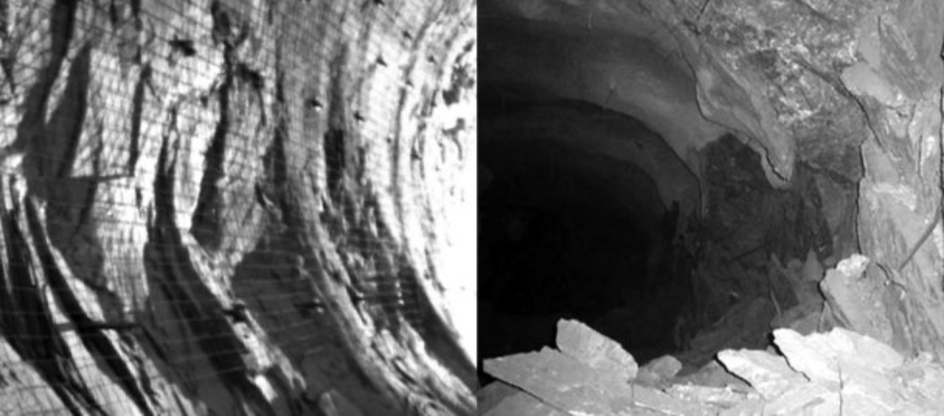
\includegraphics[scale = 1]{0409-foto ruptura por spalling.pdf}
	\end{center}
	\caption{\label{foto_spalling}À esquerda uma seção remanescente após moderada fragmentação e quebra em um túnel escavado com TBM e à direita uma seção em que parte do contorno apresentou instabilidade (flambagem) em um túnel escavado de forma não mecanizada (fonte: \citeonline[p. 1084]{Diederichs2007})}
\end{figure}

Já o \textit{Squeezing} é um modo de falha relacionado ao cisalhamento e encontrado principalmente em túneis profundos em condições de grandes tensões \textit{in situ}. Inicia-se quando a fissuração está suficientemente avançada, causando uma diminuição nas propriedades mecânicas do maciço, sem gerar instabilidade no contorno da seção. Essa diminuição das características mecânicas associada ao desenvolvimento da fissuração é progressiva e controlada, em especial, devido ao confinamento que reina no maciço. Ao contrário do primeiro mecanismo, a energia armazenada pela redistribuição das tensões é dissipada de forma gradual por deformações. Esse comportamento está intimamente relacionado com o fenômeno de fluência descrito na próxima seção a qual compreende um dos comportamentos que se pretende modelar e estudar nessa tese.

A \autoref{evolucao_convergencia} ilustra a evolução da convergência por esse fenômeno. Tal comportamento também é visto em galerias para estocagem de rejeitos radioativos em maciços argilosos profundos. Essas argilas possuem baixa condutividade hidráulica, portanto, pouca difusão molecular, sendo ideais para estocar esse material. Porém, apresentam esse comportamento diferido e que pode comprometer o projeto no longo tempo requerido para estabilização desse material radioativo. Estudos como os de \citeonline{Rousset1988} e \citeonline{Armand2013} são alguns exemplos de investigações nesse sentido. Laboratórios como o HADES na Bélgica e \textit{Meuse/Haute-Marne} (\autoref{evolucao_GED}) em Paris, são exemplos de túneis para estocagem radioativa que apresentam esse fenômeno.

\begin{figure}[H]
	\begin{center}
		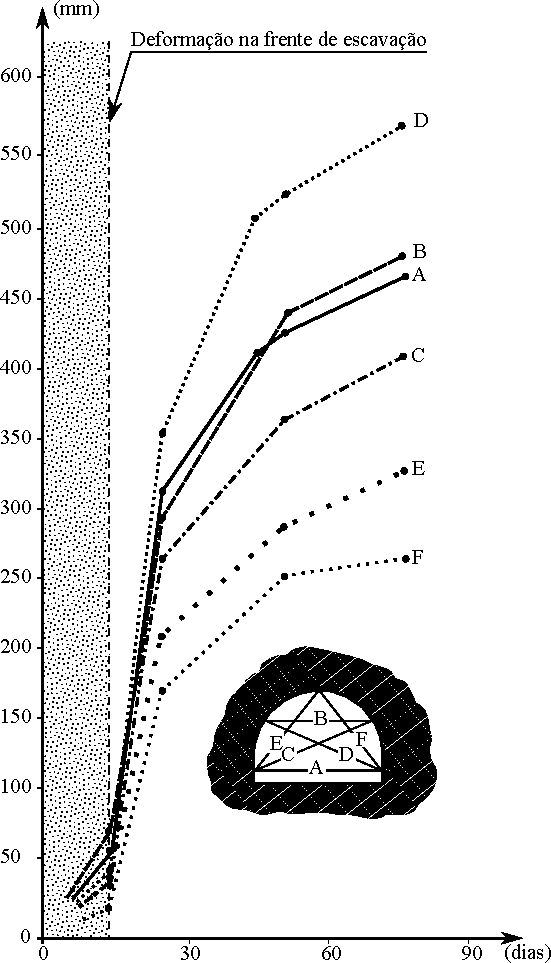
\includegraphics[scale = 1]{0410-evolução da convergencia do túnel fréjus.pdf}
	\end{center}
	\caption{\label{evolucao_convergencia}Evolução da convergência do túnel Fréjus (adaptado de: \citeonline[p. 17]{Lunardi1980})}
\end{figure}

\begin{figure}[H]
	\begin{center}
		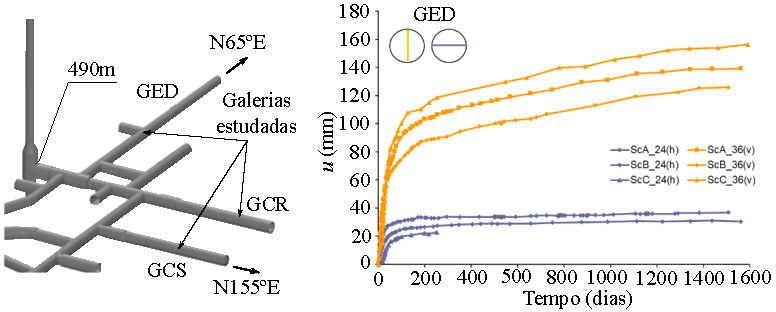
\includegraphics[scale = 1]{0411-evolucação do fechamento da seção C.pdf}
	\end{center}
	\caption{\label{evolucao_GED}Evolução do fechamento da seção GED (convergência) na galeria do laboratório \textit{Meuse/Haute-Marne}  (adaptado de: \citeonline[p. 103]{Guayacan-Carrillo2016})}
\end{figure}



\section{Influência da reologia do maciço}

\subsection{Comportamento instantâneo}

Para caracterizar o comportamento de curto prazo do maciço, o ensaio triaxial associado à medição da variação do volume é comumente utilizado. Esse ensaio clássico na mecânica das rochas permite estudar as diferentes fases do comportamento: elástica, plástica, ruptura e pós ruptura. As medidas da variação do volume permitem fazer estudos de outros aspectos do comportamento, como o coeficiente de Poisson e a dilatância. Esse ensaio, de forma resumida, consiste em submeter uma amostra cilíndrica do maciço a um estado de tensões triaxial hidrostático e, após atingido esse estado, leva-lá à ruptura através do aumento da carga axial (o desviador). \citeonline{Rousset1988}, por exemplo, caracterizou o comportamento de curto prazo de maciços argilosos profundos em frágil (argila rígida) e dúctil (argila plástica). Um maciço rígido pode ser visto na \autoref{ensaio_triaxial_rigido}.

\begin{figure}[H]
	\begin{center}
		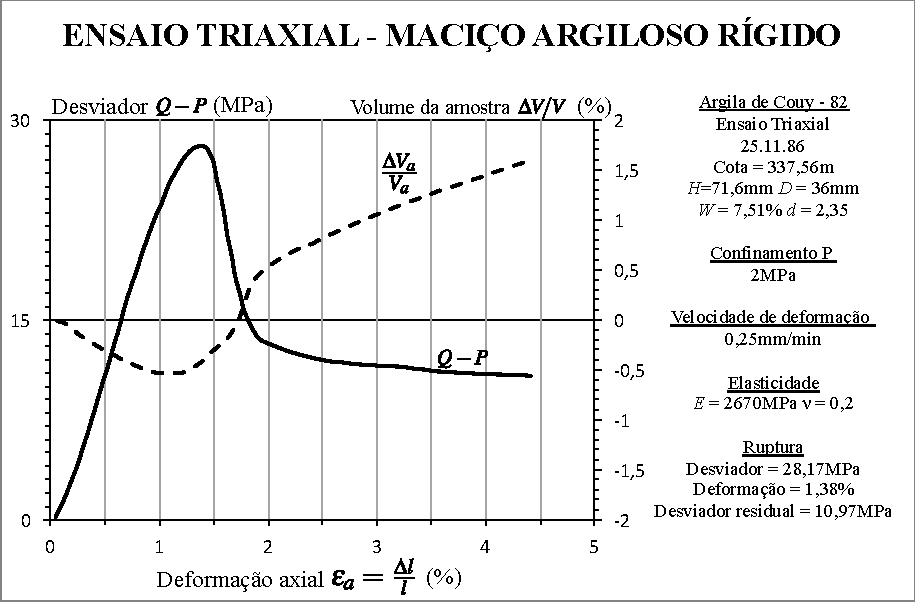
\includegraphics[scale = 0.95]{0412-ensaio triaxial argila rigida.pdf}
	\end{center}
	\caption{\label{ensaio_triaxial_rigido}Ensaio triaxial com medição da variação do volume para o caso de uma argila rígida  (adaptado de: \citeonline[p. 35]{Rousset1988})}
\end{figure}

No comportamento da \autoref{ensaio_triaxial_rigido} pode-se destacar as seguintes fases \cite[p. 34]{Rousset1988}:

\begin{alineas}
	
	\item \textbf{fase elástica} ($0\le \varepsilon \le 0,8\%$): o comportamento do maciço é linear elástico e, ao mesmo tempo, o volume da amostra diminui linearmente, os dois parâmetros elásticos, módulo de Young e Poisson, são facilmente obtidos;
	
	\item \textbf{fase pré-ruptua} ($0,8\%\le \varepsilon \le 1,3\%$): o desviador continua aumentando, mas a curva $Q-P$ não é mais linear, indicando que fenômenos irreversíveis passam a ocorrer. Ao mesmo tempo, a taxa de redução do volume diminui. Nessa fase também pode-se notar que os fenômenos irreversíveis ocorrem primeiro na curva ${\Delta V}/{V}\;$, em torno de 0,8\% da deformação enquanto o desviador é de 65\% do seu valor máximo e sua dependência ainda é linear;
	
	\item \textbf{fase de ruptura} ($1,3\%\le \varepsilon \le 1,6\%$): o desviador cai acentuadamente, o que reflete a fragilidade do comportamento dessa argila. Enquanto isso, o volume da amostra aumenta drasticamente;
	
	\item \textbf{fase pós-ruptura} ($1,6\%\le \varepsilon \le 5\%$): o desviador evoluiu pouco e mantém um valor residual de 40\% do desvio máximo. Esta resistência residual ocorre pelo atrito ao deslizamento na superfície de ruptura que apareceu durante o carregamento. Nessa fase, o volume da abertura aumenta muito, o que reflete o comportamento altamente dilatante do material (2\% superior ao volume original na deformação de 5\%).
	
\end{alineas}

Já para um maciço argiloso dúctil, o comportamento é diferente, tal como mostrado na \autoref{ensaio_triaxial_ductil}.

\begin{figure}[H]
	\begin{center}
		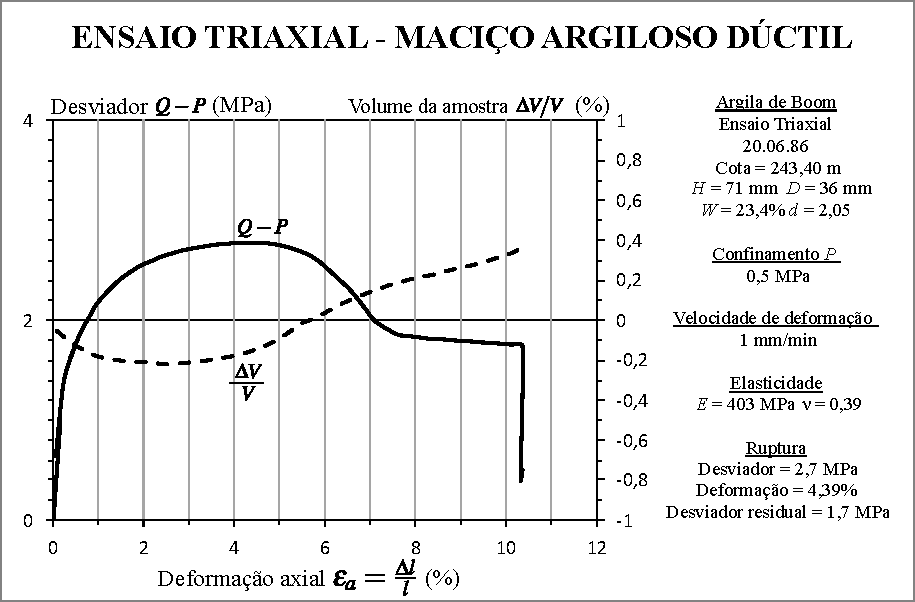
\includegraphics[scale = 0.95]{0413-ensaio triaxial argila ductil.pdf}
	\end{center}
	\caption{\label{ensaio_triaxial_ductil}Ensaio triaxial com medição da variação do volume para o caso de uma argila dúctil (adaptado de: \citeonline[p. 35]{Rousset1988})}
\end{figure}

No comportamento da \autoref{ensaio_triaxial_ductil} pode-se destacar as seguintes fases \cite[p. 35]{Rousset1988}:

\begin{alineas}
	
	\item \textbf{fase elástica} ($0\le \varepsilon \le 0,3\%$): pode-se ver que para esse caso, onde ambas as curvas são lineares, é uma fase muito pequena;
	
	\item \textbf{fase plástica com endurecimento} ($0,3\%\le \varepsilon \le 2\%$): durante essa fase o desviador continua a aumentar, mas a uma taxa decrescente. Da mesma forma, a redução do volume também teve sua taxa diminuída, mas o comportamento segue ainda de contração;
	
	\item \textbf{fase plástica perfeita} ($2\%\le \varepsilon \le 5\%$): o desviador agora segue quase constante e o volume da amostra acompanha o comportamento. Essa fase conduz a uma deformação significativa, superior a 5\%;
	
	\item \textbf{fase plástica com amolecimento} ($5\%\le \varepsilon \le 8\%$): a resistência da amostra diminui gradualmente até um platô residual e o volume começa a aumentar;
	
	\item \textbf{fase plástica residual} ($8\%\le \varepsilon \le 10\%$): o desviador é agora novamente constante, cerca de 60\% do valor máximo. O volume da amostra aumenta sensivelmente tendo uma dilatância moderada.
	
\end{alineas}


\subsection{Comportamento diferido no tempo}

\subsection{Alguns estudos considerando leis elastoplásticas e viscoplásticas}

\section{Influência da forma da seção}

\section{Influência da profundidade do túnel}

\section{Influência da proximidade da superfície}

\section{Influência do revestimento e parâmetros adimensionais}

\section{Método convergência-confinamento}




